\section{\lr{flow\_parser}}
در این بخش روش تبدیل یک فایل
\lr{.pcap}
به یک فایل
\lr{.csv}
را توضیح می‌دهیم.\\
برای استفاده از کد، باید از آن به شکل زیر استفاده کنید. 
در این کد
\lr{pcapfiles}
و
\lr{output}
به ترتیب آدرس فایل ورودی و خروجی هستند.
گزینه‌ی \lr{raw} که به طور پیشفرض غیرفعال است را در انتها توضیح می‌دهیم. 
\begin{latin}
	\begin{verbatim}
		python3 flow_parser.py -p [--pcapfile] [--raw] -o [--output]	
	\end{verbatim}
\end{latin}
برای این که درکی از کلیت اجرای کد داشته باشید، ابتدا در تابع \lr{main}، آرگومان‌های ورودی تشخیص داده می‌شوند، سپس تابع \lr{parse\_features\_to\_dataframe} صدا زده می‌شود که این تابع با استفاده از تابع \lr{flow\_processor}، اطلاعات  آماری هر \lr{flow} را به طور جداگانه به دست آورده و در یک دیتافریم \lr{pandas} قرار می‌دهد. در انتها هم این دیتافریم در یک فایل \lr{.csv} با آدرس مورد نظر ذخیره می‌شود.\\
دو مورد از نحوه‌ی استفاده از این قطعه کد در تصاویر 
\ref{fig:flowparser:normal}
و
\ref{fig:flowparser:raw}
قابل مشاهده است.
در ادامه به توضیح نحوه‌ی کار بخش‌های مختلف کد به طور جداگانه می‌پردازیم.
\begin{figure}[h]
	\centering
	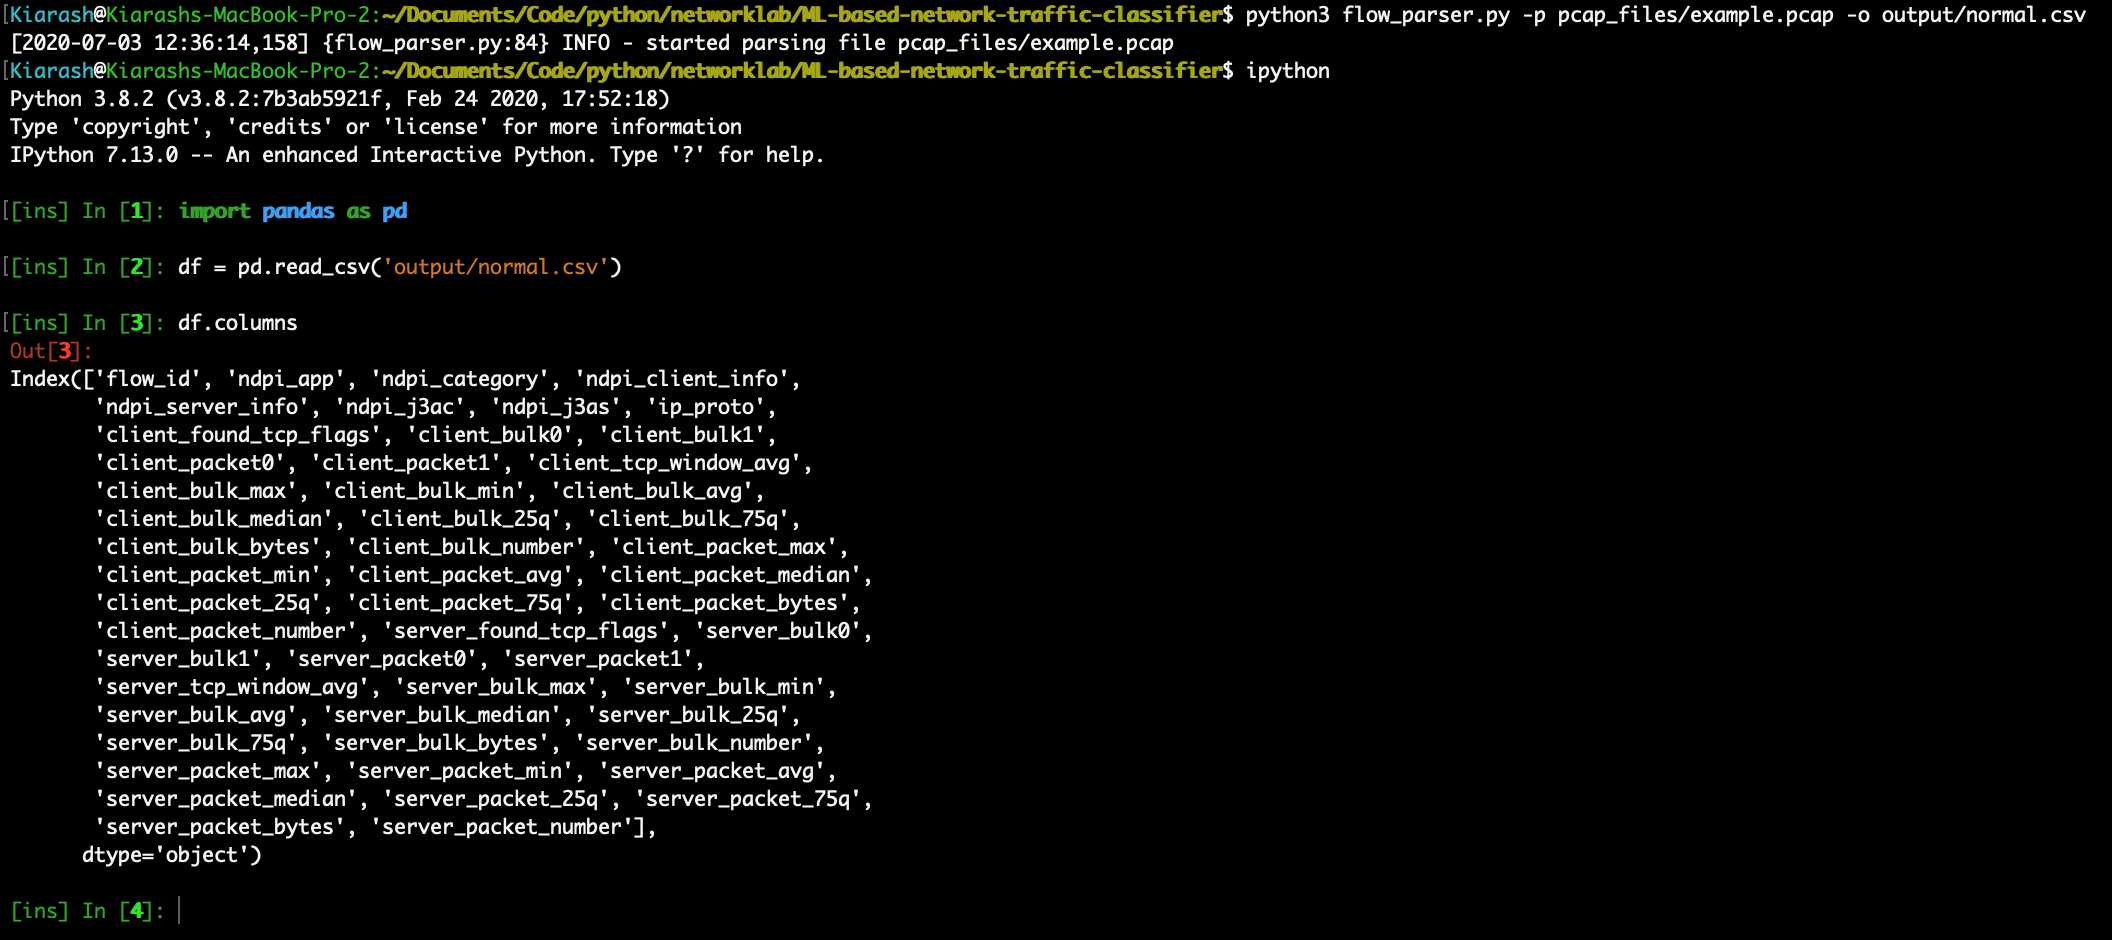
\includegraphics[width=0.6\textwidth]{data-extraction/normal}
	\caption{استفاده‌ از \lr{flow\_parser} بدون استفاده از قابلیت \lr{raw}}
	\label{fig:flowparser:normal}
\end{figure}
\begin{figure}[h]
	\centering
	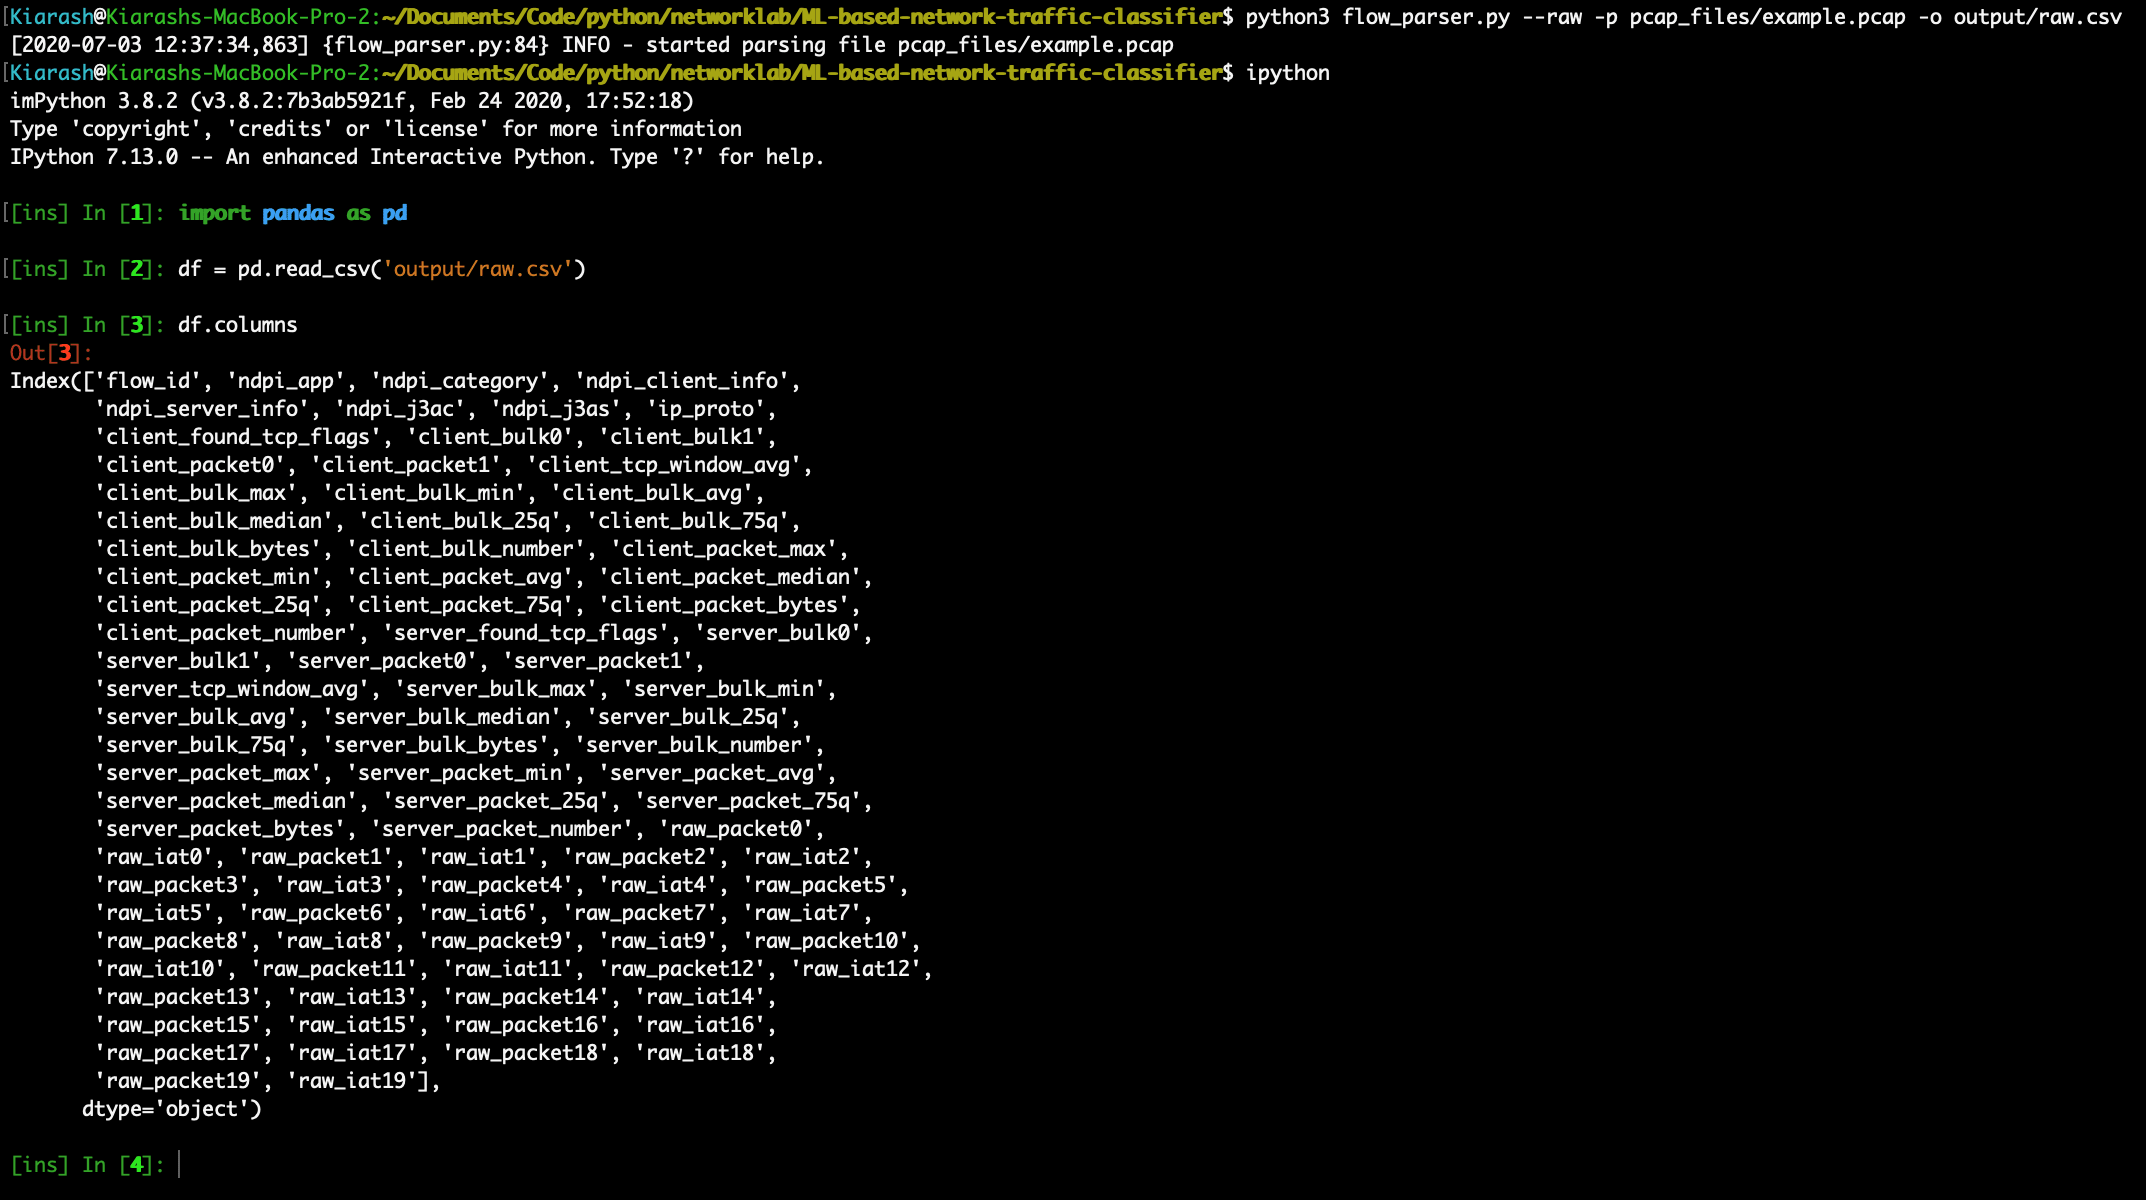
\includegraphics[width=0.6\textwidth]{data-extraction/raw}
	\caption{استفاده‌ از \lr{flow\_parser} با استفاده از قابلیت \lr{raw}}
	\label{fig:flowparser:raw}
\end{figure}
\subsection{\lr{raw\_packets\_matrix}}
این کلاس همانطور که در بخش قبل توضیح داده شد، یک زیرکلاس از \lr{nfstream.NFPlugin} است. تابع 
\lr{\_fill\_flow\_stats}
با ورودی گرفتن یک پاکت، یک ماتریس و یک شماره سطر، اطلاعات مورد نیاز این پاکت را در سطر مورد نظر از ماتریس قرار داده و خود ماتریس را خروجی می‌دهد.\\
با توجه به نحوه‌ی کار کتابخانه‌ی \lr{nfstream}، هنگامی که اولین پاکت از یک \lr{flow} مشاهده شد، تابع \lr{on\_init} از این کلاس با ورودی
\lr{obs}
که همان پاکت است صدا زده می‌شود. با این کار یک ماتریس خالی با تعداد سطر‌های کافی (بیشترین تعداد پاکت‌های ممکن در یک \lr{flow}) ساخته می‌شود که هر سطر قرار است اطلاعات یک پاکت را در خود جای دهد. این ماتریس توسط تابع خروجی داده می‌شود که باعث می‌شود که کتابخانه پس از ایجاد یک \lr{flow} از کلاس \lr{NFEntry}، مقدار 
\lr{raw\_packets\_matrix}
(نام کلاس) از این \lr{flow} را برابر با این ماتریس قرار دهد. در ادامه با مشاهده‌ی هر پاکت جدید، تابع 
\lr{on\_update}
با ورودی‌های
\lr{entry}
و
\lr{obs}
که به ترتیب نشان‌دهنده‌ی \lr{flow} و پاکت جدید هستند، مقدار ماتریس در سطر مورد نظر تغییر داده می‌شود. البته اگر تعداد پاکت‌ها آن‌قدر زیاد شده باشد که دیگر سطر خالی‌ای برای داده‌ی جدید وجود نداشته باشد، اتفاقی نمی‌افتد.\\
هنگام منقضی شدن \lr{flow} هم با صدا زدن تابع \lr{on\_expire}، سطر‌هایی از ماتریس که تمام‌صفر هستند، یعنی همان سطر‌هایی که شماره‌ی آن‌ها از تعداد بسته‌های \lr{flow} بیشتر بوده و در نتیجه اطلاعاتی در آن‌ها قرار نگرفته است، پاک می‌شوند.\\
\subsection{\lr{\_init\_streamer}}
این تابع با ورودی گرفتن آدرس یک فایل \lr{.pcap}، با استفاده از کلاس \lr{NFStreamer} و نیز 
 \lr{raw\_packets\_matrix}
 از 
\lr{NFPlugin}،
\lr{flow}‌های
فایل را استخراج کرده و آن‌ها را به شکل یک \lr{generator} خروجی می‌دهد. دقت کنید که به علت استفاده از کلاس
 \lr{raw\_packets\_matrix}،
 اطلاعاتی از پاکت‌های هر \lr{flow} که مورد نیاز ما هستند در 
 \lr{flow.raw\_packets\_matrix}
قابل دسترسی هستند.\\
\subsection{\lr{flow\_processor}}
این تابع که به نوعی مهم‌ترین تابع این بخش است و تمامی تابع‌های دیگر را به هم وصل می‌کند (به جز توابع مربوط به ریختن دیتافریم در یک فایل خروجی) با ورودی گرفتن  آدرس فایل
\lr{.pcap}،
ابتدا با استفاده از 
\lr{\_init\_streamer}،
اطلاعات خام مربوط به هر 
\lr{flow}ی
آن را به دست می‌آورد. منظور از اطلاعات خام، اطلاعات پاکت‌ها به طور جداگانه به فرم ماتریسی که قبلا توضیح داده شد و نیز اطلاعاتی از \lr{flow} که توسط کلاس \lr{NFEntry} فراهم می‌شود است.\\
در ادامه برای هر کدام از این \lr{flow}‌ها، با استفاده از تابع 
\lr{calc\_flow\_features}،
اطلاعات آماری \lr{flow} از ماتریس اطلاعات پاکت‌ها استخراج می‌شود و یک لیست که هر عضو آن اطلاعات آماری یک \lr{flow} به همراه مشخصات کلی آن است خروجی داده می‌شود.\\
\subsection{\lr{\_fill\_flow\_stats}}
این تابع اطلاعات مهم هر پاکت را از آن استخراج کرده و در سطر مناسب از ماتریس قرار می‌دهد. این اطلاعات عبارتند از برچسب زمانی پاکت، اندازه‌ی بسته‌ی لایه‌ی شبکه، اندازه‌ی محتویات پاکت، پرچم‌های \lr{TCP} پاکت در صورت وجود (برای نشان دادن این پرچم‌ها، با کنار هم قرار دادن آن‌ها، یک رشته تشکیل می‌شود که اگر در مبنای ۲ به آن نگاه کنیم، یک عدد است و این عدد را ذخیره می‌کنیم)، اندازه‌ی پنجره‌ی \lr{TCP} در صورت \lr{TCP} بودن و نیز شماره‌ی پروتوکول و جهت بسته. برای مطالعه بیشتر این مقادیر می‌توانید به جدول 
\ref{tab:NFpacket}
یا مستندات \lr{nfstream} مراجعه کنید.
\subsection{\lr{calc\_flow\_features}}
این تابع که در فایل
\lr{feature\_processing.py}
پیاده‌سازی شده است، با ورودی گرفتن یک ماتریس شامل اطلاعات پاکت‌های یک \lr{flow}، اطلاعات آماری آن را استخراج می‌کند.\\
برای این کار، ابتدا پاکت‌هایی که توسط سرور فرستاده شدند و پاکت‌هایی که توسط کلاینت فرستاده شدند از هم جدا می‌شوند.\\
سپس با استفاده از تابع
\lr{calc\_unidirectional\_flow}،
اطلاعات مربوط به هر کدام از این نوع بسته‌ها جداگانه محاسبه شده و در انتها ادغام می‌شوند.\\
برای این کار، این تابع ابتدا پرچم‌های \lr{TCP} و نیز طول میانگین پنجره‌ی \lr{TCP} را محاسبه می‌کند. سپس اطلاعات آماری هر کدام از دو ستون‌ ماتریس را که مربوط به اندازه‌ی محتویات پاکت و اندازه‌ی بسته‌ی \lr{IP} هستند را به طور جداگانه حساب می‌کند. منظور از اطلاعات آماری، مقادیری است که تابع 
\lr{calc\_parameter\_stats}
خروجی می‌دهد یعنی برای هر ستون، اولین و دومین مقدار آن (در صورت وجود)، میانگین، کمینه، بیشینه، میانه، تعداد مقادیر ناصفر، مجموع و چارک اول و چهارم.\\
\subsection{قابلیت \lr{raw}}
در صورت نیاز، می‌توان اطلاعات بیشتری را هم از 
\lr{flow}
استخراج کرد. به این منظور، هنگام استفاده از برنامه، آرگومان
\lr{raw}
باید به آن پاس داده شود. در این صورت، تابع 
\lr{flow\_processor}، 
هنگام ساخت اطلاعات هر 
\lr{flow}،
تابع 
\lr{calc\_raw\_features}
در 
\lr{feature\_processing.py}
را صدا می‌زند. این تابع هم با صدازدن توابع
\lr{\_get\_iat}
و
\lr{\_get\_packet\_features}،
به ترتیب اختلاف زمانی هر دو پاکت و نیز طول جهت‌دار هر پاکت را (یعنی اگر جهت از سرور به کلاینت باشد، عدد منفی قرار می‌دهد) را محاسبه می‌کند و به اطلاعات اضافه می‌کند. از آن‌جایی که طول
\lr{flow}‌ها
متغیر است، برای \lr{flow}‌های کوتاه‌تر، در جایگاه پاکت‌هایی که شماره‌ی آن‌ها از طول \lr{flow} بیشتر است ۰ قرار می‌گیرد.\\
